\documentclass[10pt,varwidth]{standalone}
\usepackage[a4paper, left=2.5cm, right=2.5cm, top=2.5cm, bottom=2.5cm]{geometry}
\usepackage{xifthen}
\usepackage{xfp}
\usepackage{xcolor}
\usepackage{pgfplots}
\usepackage{pgfplotstable}
\pgfplotsset{compat=1.16}
% 2.引用的tikz库
\usetikzlibrary {matrix, chains, trees, decorations}
\usetikzlibrary {arrows.meta, automata,positioning}
\usetikzlibrary {decorations.pathmorphing, calc}
\usetikzlibrary {calligraphy}
\usetikzlibrary {backgrounds, mindmap,shadows}
\usetikzlibrary {patterns, quotes, 3d, shadows}
\usetikzlibrary {graphs, fadings, scopes}
\usetikzlibrary {arrows, shapes.geometric}
\usepgflibrary {shadings}
\tikzset{
  >={Latex}
}


\begin{document}
\thispagestyle{empty}
\centering
\;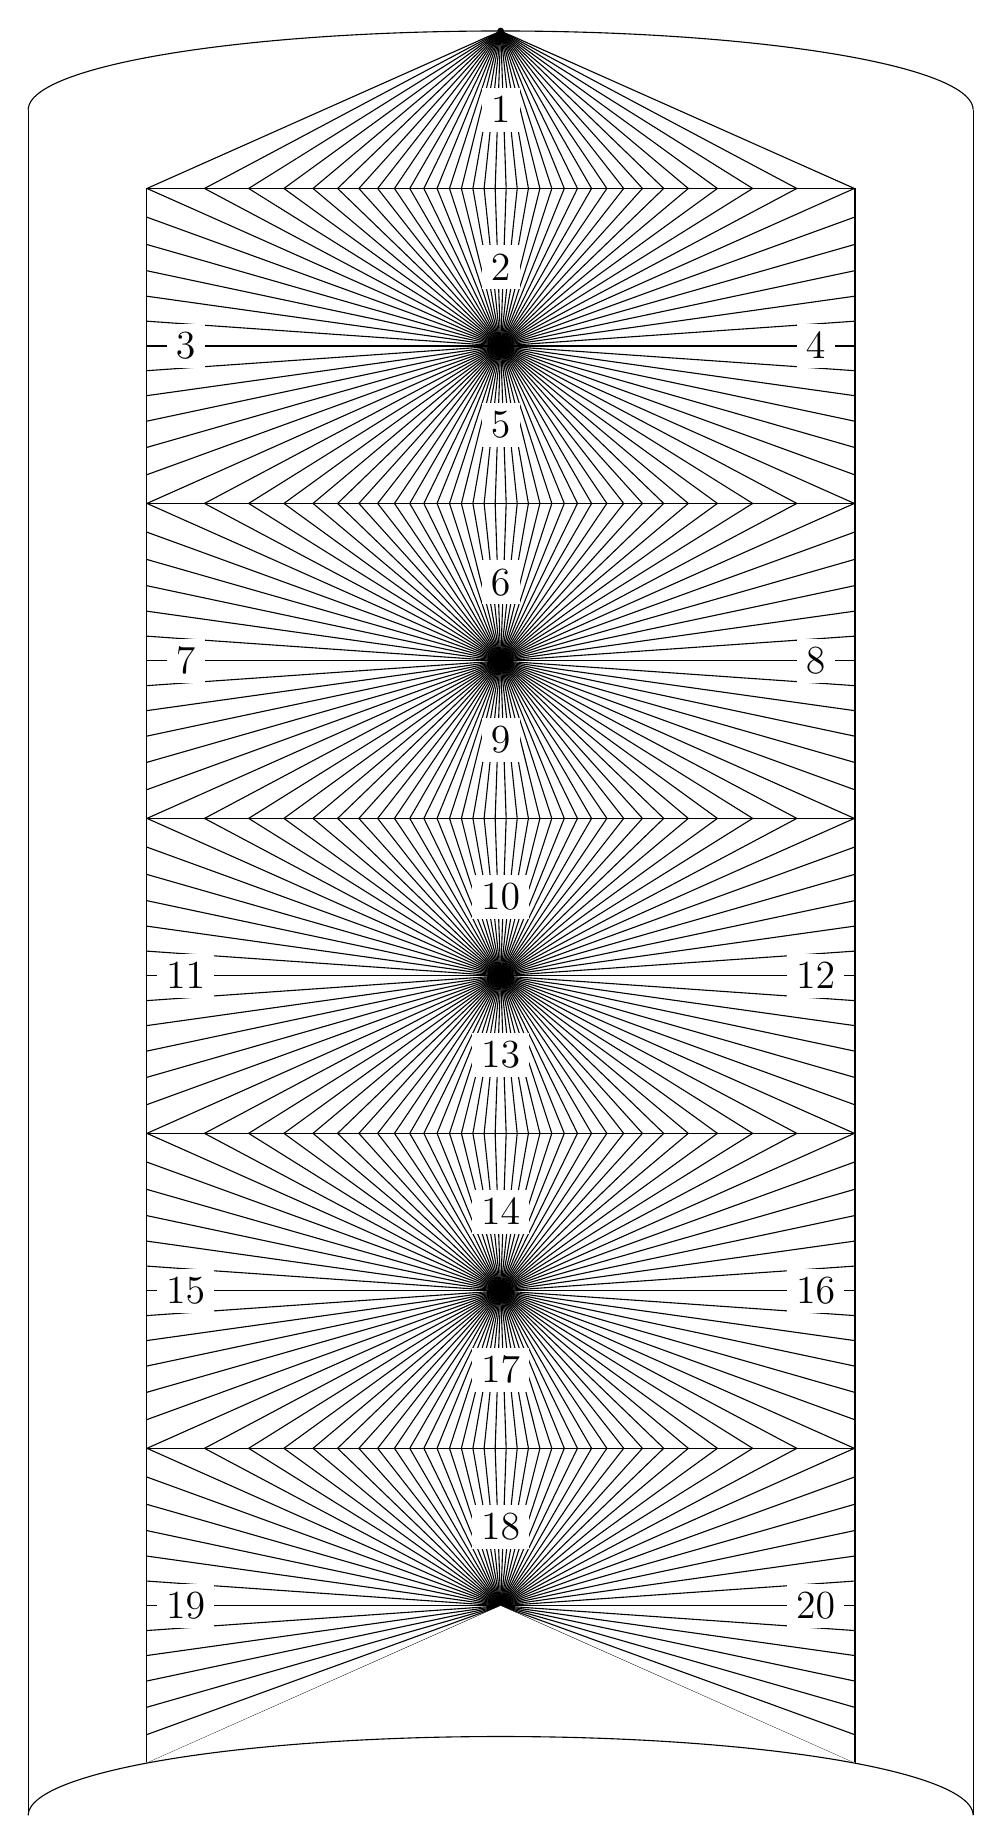
\begin{tikzpicture}[font=\Large]
    % element
    % 1.
    \begin{scope}
        \draw (-4.5, 9) -- (4.5, 9);
        \clip (0, 11) -- (-5, 9) -- (5, 9);
        \foreach \theta in {0, 4, 8, ..., 356}{
            \draw (0, 11) -- ++(\theta:8);
        } 
        \node[preaction={fill, white}] at (0, 10) {$1$};
    \end{scope}
    % 1. height of rectengle=4
    \begin{scope}
        \draw (-4.5, 5) rectangle ++(9, 4);
        \clip (-4.5, 5) rectangle ++(9, 4);
        \foreach \theta in {0, 4, 8, ..., 360}{
            \draw (0, 7) -- ++(\theta:8);
        } 
        \node[preaction={fill, white}] at (0, 8) {$2$};
        \node[preaction={fill, white}] at (0, 6) {$5$};
        \node[preaction={fill, white}] at (-4, 7) {$3$};
        \node[preaction={fill, white}] at (4, 7) {$4$};
    \end{scope}
    % 2.
    \begin{scope}[yshift=-4cm]
        \draw (-4.5, 5) rectangle ++(9, 4);
        \clip (-4.5, 5) rectangle ++(9, 4);
        \foreach \theta in {0, 4, 8, ..., 360}{
            \draw (0, 7) -- ++(\theta:8);
        } 
        \node[preaction={fill, white}] at (0, 8) {$6$};
        \node[preaction={fill, white}] at (0, 6) {$9$};
        \node[preaction={fill, white}] at (-4, 7) {$7$};
        \node[preaction={fill, white}] at (4, 7) {$8$};
    \end{scope}
    % 3.
    \begin{scope}[yshift=-8cm]
        \draw (-4.5, 5) rectangle ++(9, 4);
        \clip (-4.5, 5) rectangle ++(9, 4);
        \foreach \theta in {0, 4, 8, ..., 360}{
            \draw (0, 7) -- ++(\theta:8);
        } 
        \node[preaction={fill, white}] at (0, 8) {$10$};
        \node[preaction={fill, white}] at (0, 6) {$13$};
        \node[preaction={fill, white}] at (-4, 7) {$11$};
        \node[preaction={fill, white}] at (4, 7) {$12$};
    \end{scope}
    % 4.
    \begin{scope}[yshift=-12cm]
        \draw (-4.5, 5) rectangle ++(9, 4);
        \clip (-4.5, 5) rectangle ++(9, 4);
        \foreach \theta in {0, 4, 8, ..., 360}{
            \draw (0, 7) -- ++(\theta:8);
        } 
        \node[preaction={fill, white}] at (0, 8) {$14$};
        \node[preaction={fill, white}] at (0, 6) {$17$};
        \node[preaction={fill, white}] at (-4, 7) {$15$};
        \node[preaction={fill, white}] at (4, 7) {$16$};
    \end{scope}
    % 5.
    \begin{scope}[yshift=-16cm]
        \draw (-4.5, 5) -- ++(0, 4) -- ++(9, 0) -- ++(0, -4);
        \clip (-4.5, 5) rectangle ++(9, 4);
        \foreach \theta in {0, 4, 8, ..., 360}{
            \draw (0, 7) -- ++(\theta:8);
        } 
        \node[preaction={fill, white}] at (0, 8) {$18$};
        \node[preaction={fill, white}] at (-4, 7) {$19$};
        \node[preaction={fill, white}] at (4, 7) {$20$};
        % cover it
        \fill[white] (-4.5, 5) -- ++(9, 0) -- ++(-4.5, 2);
        \draw[very thick, white] (-4.5, 5) -- ++(9, 0);
    \end{scope}
    % axis
    % \draw[->] (-8, 0) -- (8, 0); \draw[->] (0, -12) -- (0, 12);
    % frame: method 1
    % \draw (-6, 10)  to[out=60,  in=120]   (6, 10) -- (6, -10) 
    %                 to[out=120, in=60]  (-6, -10) -- (-6, 10)
    %                 -- cycle;
    % frame: method 2
    \draw plot[samples=100,domain=0:180,smooth,variable=\t] ({6*cos(\t)}, {sin(\t)+10});
    \draw plot[samples=100,domain=0:180,smooth,variable=\t] ({6*cos(\t)}, {sin(\t)-11.66});
    \draw (6, 10) -- (6, -11.66);
    \draw (-6, 10) -- (-6, -11.66);
    \filldraw (0, 11) circle (1pt); 
\end{tikzpicture}
\end{document}